%COMSOL Multiphysics was used to develop a finite element model of the electrolyte-gated carbon nanotube field-effect transistor (EG-CNTFET) with the aim of gaining insight into the electrical and ionic transport mechanisms within the device. A schematic representation of the simulated geometry is shown in Figure~\ref{fig:comsol_geometry}, and the key parameters used in the model are summarized in Table~\ref{tab:model_parameters}. The simulation accounted for both the electrolyte and the semiconductor, that were assigned to two different domains, enabling the study of charge carrier modulation in response to ion concentration changes.

A simulation method was used with COMSOL Multiphysics to support the experimental data and obtain a better understanding of the underlying physical phenomena governing EG-CNTFETs. This software was chosen for its flexibility in handling coupled multiphysics problems, including those involving electrochemical systems. An electrochemical model was developed to simulate the behavior of the device under varying electrical conditions, with the aim of correlating theoretical predictions with the experimental data obtained during previous measurements. The simulations aimed to shed light on the mechanisms of charge modulation, ion transport, and ultimately device performance by simulating the key elements of the device architecture and operating conditions.

\begin{figure}
    \centering
    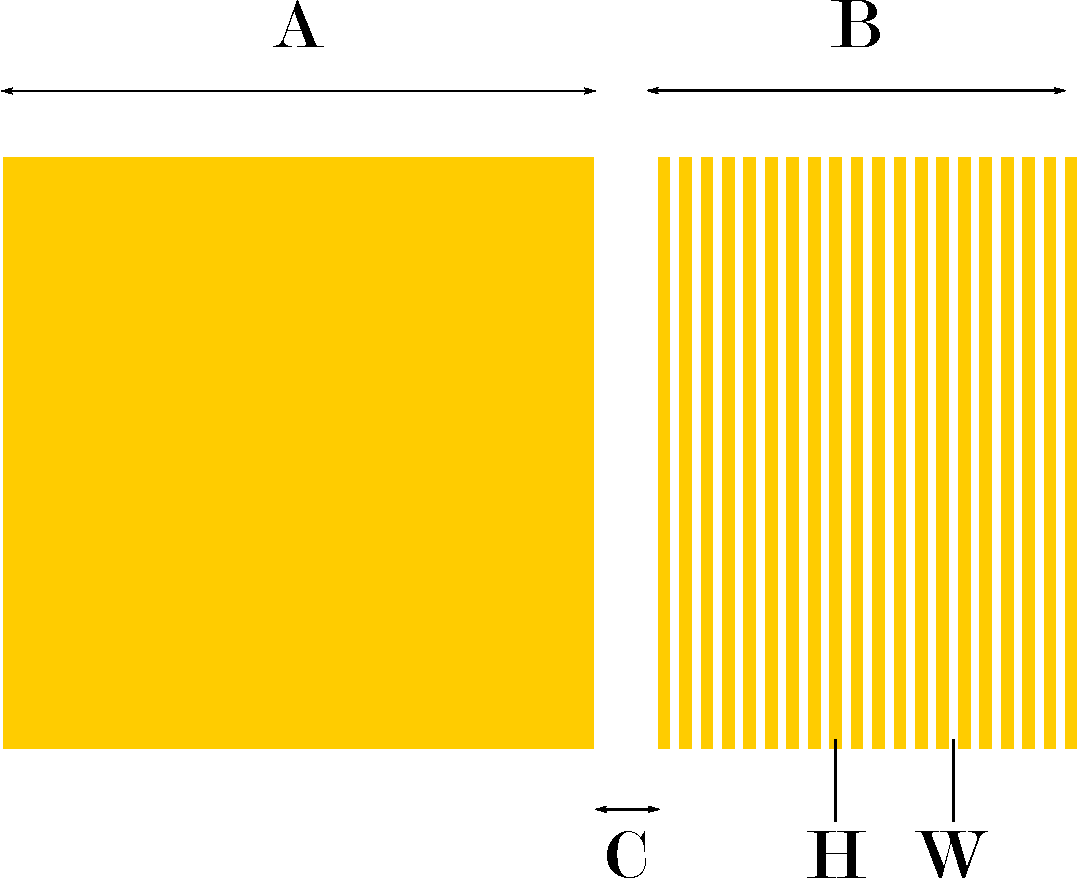
\includegraphics[width = 0.4\textwidth]{figures/chapter5/structure_params.pdf}
    \caption{Geometry of the simulated device. The values of the parametrs shown are in Table \ref{tab:model_parameters}.}
    \label{fig:simulParams}
\end{figure}

The simulated structure, illustrated in Figure~\ref{fig:simulParams}, reflects the geometry of the EG-CNTFET described in the previous chapters and aims to reproduce its essential functional elements. The model consists of two primary domains, the electrolyte and the organic semiconductor layer; These regions are defined with dimensions and material properties consistent with the fabricated devices, as summarized in Table~\ref{tab:model_parameters}. The interface between the two domains plays a crucial role in the simulations, as it is where the charges accumulate and move, and should be therefore treated with particular attention. The overall geometry has been simplified to capture the key physical interactions while maintaining computational efficiency.

The simulation model was developed using the Nernst-Planck-Poisson framework, which couples the Transport of Diluted Species and Electrostatics physics interfaces. This approach enabled the description of ion migration in an electric field, diffusion, and electric field interactions within the electrolyte, as well as the electrostatic potential distribution across the device. The parameters necessary to simulate the devices, such as diffusion coefficients, charge numbers, initial concentrations, and dielectric constants, were assigned to the corresponding domains, as detailed in Table~\ref{tab:model_parameters}. Boundary conditions were applied to reflect the experimental configuration, with appropriate electric potentials set at the gate and source/drain contacts, and no-flux defined at the boundaries. These are illustrated in Figure~\ref{fig:boundaryConditions} and were chosen to replicate the actual operating environment of the EG-CNTFET.

Due to the coupled and nonlinear nature of the model, a fully coupled stationary solver was employed. Solver settings, including convergence tolerances and damping strategies, are still being tuned, as mesh refinement is still ongoing. Future steps may also involve time-dependent simulations, depending on the desired insights into transient behaviors.

The simulations are intended to provide insight into key physical parameters of the EG-CNTFET device, including the electrostatic potential distribution, ion concentration profiles, charge accumulation at the interface. These results are expected to complement the experimental findings by offering a theoretical understanding of how device geometry, material properties, and boundary conditions influence sensing performance. Ultimately, this approach supports the interpretation of experimental trends and guides further device optimization.

At the current stage, the simulation framework has been set up, and all relevant physical parameters and boundary conditions have been defined. However, the main challenge remains the optimization of the mesh, that still has not been able to fully contribute to the description of the behaviour of the device. The next steps will focus on resolving these meshing issues and subsequently validating the model against preliminary experimental data.

\begin{table}[htbp]
    \centering
    \caption{Model parameters}
    \begin{tabular}{lll}
    \toprule
    \textbf{Parameter} & \textbf{Value} & \textbf{Description} \\
    \midrule
    $A$ & 5.7~mm &  \\
    $B$ & 2.25~mm &  \\
    $C$ & 1.5~mm &  \\
    $c_0$ & 138~mol/m$^3$ &  \\
    $D_a$ & $2.03 \times 10^{-9}$~m$^2$/s & Diffusion coefficient of anions \\
    $D_c$ & $1.33 \times 10^{-9}$~m$^2$/s & Diffusion coefficient of cations \\
    $D_p$ & $5.04 \times 10^{-8}$~m$^2$/s & Diffusion coefficient of holes \\
    $E_b$ & 0.2~eV &  \\
    $\varepsilon_{\text{el}}$ & 79 & Dielectric constant of the electrolyte \\
    $\varepsilon_{\text{OSC}}$ & 3 & Dielectric constant of the semiconductor \\
    $H$ & 100~$\mu$m & Source-Drain height \\
    $L$ & 50~$\mu$m & Channel length \\
    $W$ & 57~mm &  Channel width \\
    $L_e$ & 100~$\mu$m & Electrolyte thickness \\
    $L_s$ & $5 \times 10^{-7}$~m & Semiconductor thickness \\
    $\mu_{\text{hole}}$ & 30~cm$^2$/V$\cdot$s & Hole mobility $\mu_p$ \\
    $T$ & 293~K &  \\
    $V_{\text{dr}}$ & 0~V & $V_{\text{DS}}$ \\
    $V_g$ & 0~V & $V_{\text{GS}}$ \\
    $z_a$ & $-1$ & Charge of anions \\
    $z_c$ & $+1$ & Charge of cations \\
    $z_p$ & $+1$ & Charge of holes \\
    $D_h$ & $k_B \cdot T \cdot \mu_{\text{hole}} / e$ &  \\
    $ch_0$ & $1 \times 10^{-7}$~mol/m$^3$ & Initial hole concentration \\
    \bottomrule
    \end{tabular}
    \label{tab:model_parameters}
\end{table}


    